\documentclass[a4paper]{article}

\usepackage[english]{babel}
\usepackage{amsmath}
\usepackage{color}
\usepackage{amssymb}
\usepackage{dsfont}
\usepackage{multicol}
%\usepackage[lofdepth,lotdepth]{subfig}  This gives errors when used together with "subcaption", which is needed to create subfigures.
\usepackage{graphicx}
\usepackage{listings}
\usepackage[hyphens]{url}
\usepackage{pgf, tikz}
\usetikzlibrary{arrows, automata}
\usepackage{titling}
\usepackage{varwidth}
\usepackage{hyperref}
\usepackage{color} %red, green, blue, yellow, cyan, magenta, black, white
\definecolor{mygreen}{RGB}{28,172,0} % color values Red, Green, Blue
\definecolor{mylilas}{RGB}{170,55,241}
\setlength\parindent{0pt}
\usepackage{float}
\usepackage{subcaption}
\usepackage{polynom}
\usepackage{physics}



\newcommand\independent{\protect\mathpalette{\protect\independenT}{\perp}}
\def\independenT#1#2{\mathrel{\rlap{$#1#2$}\mkern2mu{#1#2}}}

\usepackage{geometry}
 \geometry{
 a4paper,
 total={165mm,257mm},
 left=20mm,
 top=20mm,
 }

\definecolor{codegreen}{rgb}{0,0.6,0}
\definecolor{codegray}{rgb}{0.5,0.5,0.5}
\definecolor{codepurple}{rgb}{0.58,0,0.82}
\definecolor{backcolour}{rgb}{0.95,0.95,0.92}

\lstdefinestyle{mystyle}{
    backgroundcolor=\color{backcolour},   
    commentstyle=\color{codegreen},
    keywordstyle=\color{magenta},
    numberstyle=\tiny\color{codegray},
    stringstyle=\color{codepurple},
    basicstyle=\footnotesize,
    breakatwhitespace=false,         
    breaklines=true,                 
    captionpos=b,                    
    keepspaces=true,                 
    numbers=left,                    
    numbersep=5pt,                  
    showspaces=false,                
    showstringspaces=false,
    showtabs=false,                  
    tabsize=2
}
 
\lstset{style=mystyle}


\DeclareMathOperator*{\argmax}{arg\,max}
\DeclareMathOperator*{\argmin}{arg\,min}

\title{Statistical Machine Learning 2018\\Assignment 3\\Deadline: 25th of November 2018}
\author{
  Christoph Schmidl\\ s4226887\\      \texttt{c.schmidl@student.ru.nl}
  \and
  Mark Beijer\\ s4354834\\     \texttt{mbeijer@science.ru.nl}
}
\date{\today}

\begin{document}
\maketitle


\section*{Exercise 1 - The faulty lighthouse (weight 5)}

A lighthouse is somewhere off a piece of straight coastline at a position $\alpha$ along the shore and a distance $\beta$ out to sea. Due to a technical fault, as it rotates the light source only occasionally and briefly flickers on and off. As a result it emits short, highly focused beams of light at random intervals. These pulses are intercepted on the coast by photo-detectors that record only the fact that a flash has occurred, but not the angle from which it came. So far, $N$ flashes have been recorded at positions $\mathcal{D} = {x1, . . . , xN }$. Where is the lighthouse?

\begin{figure}[H]
\center
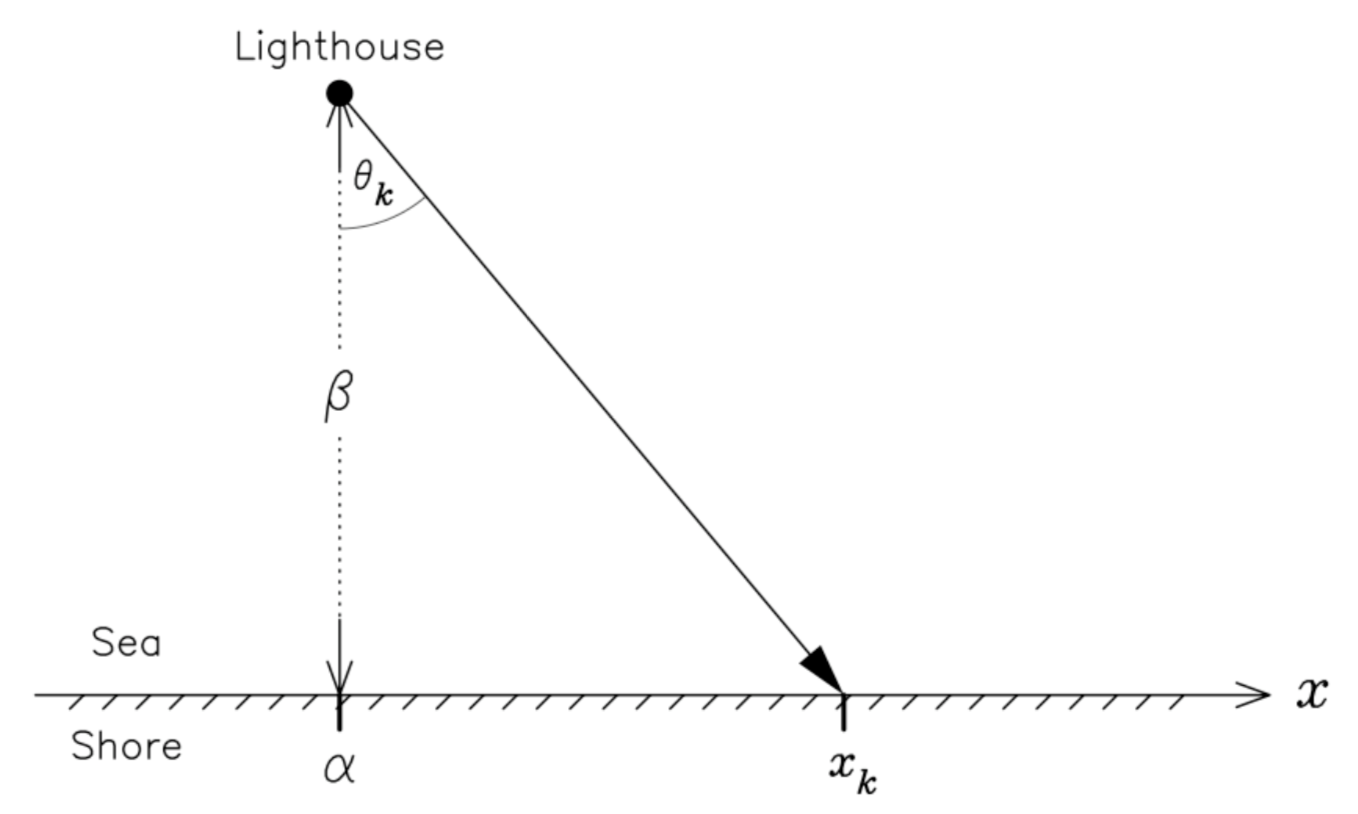
\includegraphics[width=0.75\textwidth]{Images/lighthouse_fig.png}
\caption{Geometry of the lighthouse problem.}
\label{Fig:lighthouse}
\end{figure}




\textbf{Part 1 - Constructing the model}\\

\subsection*{1.1.1}

Let $\theta_k$ be the (unknown) angle for the k-th recorded flash, see fig.1. Argue why

\begin{eqnarray}
p(\theta_k | \alpha, \beta) = \frac{1}{\pi}
\end{eqnarray}

would be a reasonable distribution over $\theta_k$ between $\pm \frac{\pi}{2}$ (zero otherwise).\\


\textbf{Answer:}\\



\subsection*{1.1.2}

We only have the position $x_k$ of the detector that recorded flash $k$, but we can relate this to the unknown $\theta_k$ via elementary geometry as

\begin{eqnarray}
\beta \tan(\theta_k) = x_k - \alpha	
\end{eqnarray}

Show that the expected distribution over $x$ given $\alpha$ and $\beta$ can be written as

\begin{eqnarray}
p(x_k | \alpha, \beta) = \frac{\beta}{\pi [\beta^2 + (x_k - \alpha)^2 ]}
\end{eqnarray}

by using (2) to substitute variable $x_k$ for $\theta_k$ in the distribution (1). Plot the distribution for $\beta = 1$ and a particular value of $\alpha$.\\
Hint: use the Jacobian $|\frac{d \theta}{d x }|$ (Bishop, p.18) and the fact that $(tan^{-1}x)' = \frac{1}{1 + x^2}$.\\



\textbf{Answer:}\\



\subsection*{1.1.3}

Inferring the position of the lighthouse corresponds to estimating $\alpha$ and $\beta$ from the data $\mathcal{D}$. This is still quite difficult, but if we assume that $\beta$ is known, then from Bayes’ theorem we know that $p(\alpha|\mathcal{D}, \beta) \propto p(\mathcal{D}|\alpha, \beta) p(\alpha|\beta)$. We have no a priori knowledge about the position $\alpha$ along the coast other than that it should not depend on the distance out at sea.\\

Show that with these assumptions the log of the posterior density can be written as

\begin{eqnarray}
L = \ln (p(\alpha | \mathcal{D, \beta})) = \texttt{constant} - \sum_{k = 1}^N \ln [\beta^2 + (x_k - \alpha)^2] 
\end{eqnarray}

and give an expression for the value $\hat{\alpha}$ that maximizes this posterior density.\\

\textbf{Answer:}\\


\subsection*{1.1.4}

Suppose we have a data set (in km) of $\mathcal{D} = \{ 3.6, 7.7, -2.6, 4.9, -2.3, 0.2, -7.3, 4.4, 7.3, -5.7\}$. We also assume that the distance $\beta$ from the shore is known to be 2 km. As it is difficult to find a simple expression for the value of $\hat{\alpha}$ that maximizes (4), we try an alternative approach instead.\\

Plot $p(\alpha|\mathcal{D}, \beta = 2)$ as a function of $\alpha$ over the interval $[-10, 10]$. What is your most likely estimate for $\hat{\alpha}$ based on this graph? Compare with the mean estimate of the dataset. Can you explain the difference?\\


\textbf{Answer:}\\




\textbf{Part 2 - Generate the lighthouse data}\\


We will try to solve the original problem by letting matlab/Python find the lighthouse for us. For that we first need a data set.

\subsection*{1.2.1}

Sample a random position $(\alpha_t, \beta_t)$ from a uniform distribution over an interval of 10 km along the coast and between 2 and 4 km out to sea.\\

\textbf{Answer:}\\


\subsection*{1.2.2}

From this position generate a data set $\mathcal{D} = \{ x_1,..., x_N \}$ of 500 flashes in random directions that have been registered by a detector at point $x_i$ along the coast. Assume that the flashes are i.i.d. according to (1).\\

\textbf{Answer:}\\


\subsection*{1.2.3}

Make a plot of the mean of the data set as a function of the number of points. Compare with the true position of the lighthouse $\alpha_t$. How many points do you expect to need to obtain a reasonable estimate of $\alpha_t$ from the mean? Explain.\\

\textbf{Answer:}\\



\textbf{Part 3 - Find the lighthouse}\\

From the analysis in the first part we know that trying to find a maximum likelihood estimate in the usual way is possible (compute gradient, set equal to zero and solve), but that this does not result in a ‘nice’ closed-form expression for the solution, even when one of the parameters is assumed to be known. As we want to find estimates of both $\alpha$ and $\beta$ from the data, we will try a different approach instead.

\subsection*{1.3.1}

Use (3) to get an expression for the loglikelihood of the data $\mathcal{D}$ as a function of $\alpha$ and $\beta$.\\

\textbf{Answer:}\\


\subsection*{1.3.2}

We can see how this likelihood (as a function of $\alpha$ and $\beta$) changes, as data points come in.\\

Process your data set $\mathcal{D}$ one by one and make a plot of the (log)likelihood after one, two, three, and 20 points have arrived, respectively. Explain what happens.\\

Hint: Create a function that calculates the (log)likelihood at a specific point $(\alpha, \beta)$ after the first $k$ data points $\{x_1, . . . , x_k \}$ have come in. Use this with the matlab \texttt{ meshgrid} and \texttt{surf}  functions to make plots over the interval $[-10 \leq \alpha \leq +10] \times [0 \leq \beta \leq 5]$. Decide if/when it makes more sense to use the likelihood directly or the log of the likelihood.\\

\textbf{Answer:}\\



\subsection*{1.3.3}

We can make a reasonable (visual) estimate of the most probable position of the lighthouse from the graph, after a few data points have been observed. However, as we are working with a computer, we will let matlab do the dirty work for us.\\

Create a function that uses matlab function \texttt{fminsearch} to compute the values of $\alpha$ and $\beta$ that maximize the likelihood for a data set of $k$ points, and plot these as a function of the number of points. Use $[0, 1]$ as the initial starting value for \texttt{ fminsearch} (see examples in matlab-help). Compare your final estimate with the true values $(\alpha_t,\beta_t)$.\\

\textbf{Answer:}\\



\section*{Exercise 2 - Bayesian linear regression (weight 2)}

This exercise builds on exercise 2, week 7, “Fitting a straight line to data”. For a detailed de- scription (and explanation) see Exercises and Answers, Week 7 in Brightspace. The final part of that exercise computed the predictive distribution after a single data point was observed. Here we consider a new data set, consisting of no less than two points: ${x_1,t_1} = (0.4,0.1)$ and ${x_2, t_2} = (0.6, -0.4)$.


\subsection*{2.1}

Assume $\alpha = 1$ and $\beta = 15$. Compute the predictive distribution $p(t|x, \textbf{t}, \textbf{x}, \alpha, \beta)$ after these two points are observed.\\

\textbf{Answer:}\\


\subsection*{2.2}


Plot the mean of the predictive Gaussian distribution and one standard deviation on both sides as a function of $x$ over the interval $[0,1]$. Plot the data in the same figure. See \texttt{a009plotideas.m} in Brightspace for some plotting hints. Compare your plot with Figure 3.8b (Bishop, p.157) and explain the difference.\\

\textbf{Answer:}\\



\subsection*{2.3}

Sample five functions $y(x,\textbf{w})$ from the posterior distribution over $\textbf{w}$ for this data set and plot them in the same graph (i.e. with the predictive distribution). You may use the Matlab function \texttt{mvnrnd}. See again \texttt{a009plotideas.m} for some plotting hints.\\

\textbf{Answer:}\\



\section*{Exercise 3 - Gradient descent revisited (weight 3)}

In this exercise, we will have a closer look at the gradient descent algorithm for function minimization. When the function to be minimized is $E(x)$, the gradient descent iteration is


\begin{eqnarray}
\textbf{x}_{n + 1} = \textbf{x}_n - \eta \nabla E(\textbf{x}_n)
\end{eqnarray}

where $\eta > 0$ is the so-called learning-rate.

\subsection*{3.1}

Consider the function $f(x) = \frac{\lambda}{2}(x - a)^2$ with parameters $\lambda > 0$, and $a$ arbitrary.


\subsection*{3.1a}

Write down the gradient descent iteration rule. Verify that the minimum of $f$ is a fixed point\footnote{A fixed point $x^*$ of an iteration $x_{n+1} = F(x_n)$ satisfies $x^* = F(x^*)$.} of the gradient descent iteration rule.\\

\textbf{Answer:}\\

The gradient of f is:

\begin{equation}
\nabla f(x) = \lambda (x-a)
\end{equation}

And therefore the gradient descent iteration rule is:

\begin{equation}
x_{n+1} = x_n - \eta \lambda (x_n-a)
\end{equation}

The minimum of f can be found by setting it's gradient to 0:

\begin{eqnarray}
\lambda(x-a) &=& 0\\
x-a &=& 0 \\
x &=& a
\end{eqnarray}

To show it's a minimum we can take the second derivitive at point a:

\begin{equation}
f''(x) = \lambda \rightarrow f''(a) = \lambda
\end{equation}

Since $\lambda$ is strictly greater then 0, the second derivative at a is strictly greater then 0 and therefor a is the minimum.

a is a fixed point since:

\begin{eqnarray}
x_{n+1} &=& a - \eta \nabla f(a)\\
&=& a - \eta \lambda (a-a) = a
\end{eqnarray}

\subsection*{3.1b}

Find $\eta$ for which convergence is the fastest (actually in one step).\\

\textbf{Answer:}\\

Since it is given that the fastest is in one step, we can write :

\begin{eqnarray}
a &=& x - \eta \lambda f(x)\\
&=& x - \eta \lambda (x-a)\\
\eta \lambda (x-a) &=& x - a\\
\eta \lambda &=& 1\\
\eta &=& \frac{1}{\lambda}
\end{eqnarray}

You can also see this by looking at the iteration rule. Since when $\eta = \lambda^{-1}$, in the next iteration $x_n$ will cancel and you're left with (-(-a))=a, thus arriving at the minimum in one step, independent of x. 

\subsection*{3.1c}

We will investigate the convergence properties for different values of $\eta$. For this we look at the ratio of the distance to the fixed point after the step and the distance before the step:
 
\begin{eqnarray}
r_n = \frac{|x_{n+1} - x^*|}{|x_n - x*|}
\end{eqnarray}

\subsubsection*{3.1c.i}

What does it mean if all $r_n < c < 1$ (i.e. all ratio’s are smaller than a certain number below 1). Give for this case the (optimal) upper bound of the distance $|x_n - x^*|$ in terms of $|x_0 - x^*|$ , $c$ and $n$.\\

\textbf{Answer:}\\

If for all $r_n < c < 1$ then it means that always, independent of the iteration step, beginning starting point $x_0$, the ratios of the next iteration and the current are always lower then some number strictly smaller then 1. This means that the distance $r_n$ to the fixed point always decreases with a rate bounded by c. It also means that every new step brings you closer to a, it's not like there is some other fixed point you might end up at.
\newpage 
At every step the distance is multiplied by at least c, since the difference between the distance of the current and next step is c or lower. So the upper bound on the distance would be:

\begin{equation}
\abs{x_n-x^*} = c^n \abs{x_0 - x^{*}}
\end{equation}

Note that $c^n < 1$ since $ 0 < c < 1$.


\subsubsection*{3.1c.ii}

What is the consequence if all $r_ > c > 1$? Give for this case the optimal lower bound of the distance $|x_n - x^*|$ in terms of $|x_0 - x^*|$, $c$ and $n$.\\

\textbf{Answer:}\\


Then with every step you get further and further away from the optimal point $x^*$. Therefore you'll diverge from the point $x^*$. while $r_c$ would be strictly greater then 1, any value just slightly higher then 1 is reachable in n steps. Thus 

\subsection*{3.1d}

Show that in our case, $r_n = |1 - \eta \lambda| \equiv r$, independent of $n$ (we refer to $r$ as the convergence rate). For which $\eta$ is the algorithm convergent?\\

\textbf{Answer:}\\



\subsection*{3.2}

Consider the function $g(x, y) = \frac{\lambda_1}{2}(x - a_1)^2 + \frac{\lambda_2}{2} (y - a_2)^2$ with parameters $0 < \lambda_1 \leq \lambda_2$, and $a_i$ arbitrary.

\subsection*{3.2a}

Write down the gradient descent iteration rule. Verify that the minimum of $f$ is a fixed point.\\

\textbf{Answer:}\\


\subsection*{3.2b}

Show that $\eta = \frac{2}{\lambda_2 + \lambda_1}$ minimizes the larger ratio between $r_{n,x} = \frac{|x_{n+1} - x^*|}{|x_n - x^*|}$ and 	$r_{n,y} = \frac{|y_{n+1} - y^*|}{|y_n - y^*|}$, i.e., $\argmin_\eta \{ max\{r_{n,x},r_{n,y} \} \} = \frac{2}{\lambda_2 + \lambda_1}$. What happens if $\eta$ is smaller than this optimal value? What happens if it is larger?\\

\textbf{Answer:}\\

\subsection*{3.2c}

What is the convergence rate for this $\eta$? What does this say about the applicability of
gradient descent to functions with steep hills and flat valleys (i.e., if $\lambda_2 \gg \lambda_1$)?\\

\textbf{Answer:}\\


\subsection*{3.2d}

Implement the gradient descent algorithm for g in matlab.\\

\textbf{Answer:}\\


\subsection*{3.2e}

Make some plots of the trajectories $\{(x_n,y_n)\}^N_{n=0}$ for different values of $\lambda_i$ and $\eta$ ($\eta$ optimal, larger than optimal, and smaller than optimal) to illustrate what is going on. Plot these trajectories on top of a contour plot of g. Monitor the convergence rates. Explain what happens.\\

\textbf{Answer:}\\



\end{document}
